\documentclass{article}
\usepackage{graphicx} % Required for inserting images
\usepackage{geometry}
 \geometry{
 left=35mm,
 right = 35mm,
 top=30mm,
 }
\usepackage{pgfplots}
\usepackage{mathrsfs}
\usepackage{wrapfig}
\usepackage{amsmath}
\usepackage{tikz}
\pgfplotsset{compat=1.18}
\usepackage{listings}
\usepackage{minted}
\usetikzlibrary{decorations.pathmorphing,calc}

\colorlet{mygold}{yellow!50!orange}
\colorlet{mydarkgold}{yellow!20!orange}
\colorlet{mylightyellow}{yellow!15!white}
\colorlet{mylightblue}{blue!35!white}
\colorlet{mylightred}{red!35!white}
\colorlet{mylightestred}{red!10!white}
\colorlet{mylightestblue}{blue!5!white}
\colorlet{mydarkpurple}{blue!40!red!50!black}
\colorlet{mydarkgreen}{green!50!black}
\colorlet{mylightpurple}{purple!5!white}
\colorlet{mydarkblue}{blue!65!black}
\colorlet{mydarkred}{red!65!black}
\colorlet{mygreen}{green!60!black}


% Credit to https://tikz.net/relativity_penrose_diagram/ for styling:


\tikzset{>=latex} % for LaTeX arrow head
\tikzstyle{photon}=[-{latex},mygold,line width=0.4,decorate,
                    decoration={snake,amplitude=0.9,segment length=4,post length=3.8}]
\tikzstyle{cone}=[mydarkblue,line width=0.2,top color=blue!60!black!30,
                  bottom color=blue!60!black!50!red!30,shading angle=60,fill opacity=0.9]
\tikzstyle{cone back}=[mydarkblue,line width=0.1,dash pattern=on 1pt off 1pt]
\tikzstyle{singularity}=[red!80!black,line width=0.8,decorate,
                         decoration={zigzag,amplitude=2,segment length=6.17}]

% LIGHTCONE
\def\R{0.25} % size lightcone
\def\e{0.25} % vertical scale
\def\ang{45} % angle light cone
\def\angb{acos(sqrt(\e)*sin(\ang))} % angle ellipse center to point of tangency
\def\a{\R*sin(\ang)*sqrt(1-\e*sin(\ang)^2)/(1-\e*sin(\ang)^2)} % vertical radius
\def\b{\R*sqrt(\e)*sin(\ang)*cos(\ang)/(1-\e*sin(\ang)^2)} % horizontal radius
\def\coneback#1{ % light cone part to be drawn behind world lines
  \draw[cone back] % dashed line back
    (#1)++(-45:\R) arc({90-\angb}:{90+\angb}:{\a} and {\b});
  \draw[cone,shading angle=-60] % top edge & inside
    (#1)++(0,{\R*cos(\ang)/(1-\e*sin(\ang)^2)}) ellipse({\a} and {\b});
}
\def\conefront#1{ % light cone part to be drawn over world lines
  \draw[cone] % light cone outside
    (#1) --++ (45:\R) arc({\angb-90}:{-90-\angb}:{\a} and {\b})
     --++ (-45:2*\R) arc({90-\angb}:{-270+\angb}:{\a} and {\b}) -- cycle;
}

% https://stackoverflow.com/questions/71250604/aps-citation-style-in-latex

\usepackage[%
    style=phys,%
    articletitle=false,biblabel=brackets,%
    chaptertitle=false,pageranges=false%
]{biblatex}
\addbibresource{citations.bib}

\title{Penrose Diagrams for Black Holes}
\author{Dwaipayan Chanda, PHYS 430}
\date{April 2024}

\begin{document}
\maketitle

\section{Introduction}
In general relativity, spacetime diagrams are one of the most versatile and insightful tools to help visualize the nature of a spacetime. We use them to interpret complex spacetimes and lorentz frames, providing us a more intuitive geometric interpretation for these problems.

There is, however, a fundamental limitation to the general spacetime diagram: \textit{its extent is infinite}. This makes sense---space and time extend to their respective positive and negative infinities, after all (except in the radial case, where space extends from 0 to positive infinity). This property, however, can make reasoning with complicated spacetimes quite difficult.

Imagine, however, a diagram where these spacelike and timelike infinities are visualized a \textit{finite} boundaries, similar to how the coordinate axes serve as an indication of where coordinates tend towards zero. One may envision how general relativity (GR), which often deals with spacelike and timelike infinities in the context of black holes, may have use for such a visual representation.

Introducing: the \textbf{Penrose Diagram} (also called the \textit{conformal diagram}). Conceptualized by mathematical physicist Robert Penrose in the 1950s, this method of visualizing a spacetime performs this exact task of ``compactifying" an infinite spacetime using functions that map infinite domains onto finite ranges \cite{minkowski_penrose_desc}. In making these transformations, however, the Penrose diagram not only preserves important properties of the spacetime (and several fundamental characteristics of GR as a whole), but also provides a useful visual tool to visualize what occurs at the infinite boundaries of a spacetime that are otherwise impossible to realize on a typical spacetime diagram.

In this paper, I will describe the characteristics of these incredibly useful diagrams, demonstrate how to generate them, derive the coordinate transformations used to map them for several example spacetimes, and finally illustrate their utility in revealing useful insights into the nature of spacetimes.

\section{Creating a Penrose Diagram}

Creating a Penrose diagram from a general spacetime diagram (which I will henceforth call a GSD) for a particular spacetime performs two main operations:

\begin{enumerate}
    \item \textbf{``Compactification"} of spacetime infinities onto finite intervals.
    \item Preserving of the property that lightlike geodesics are always at $45^{\circ}$ angles with respect to the axes.
\end{enumerate}

In doing so, it preserves the important properties of a GSD that define spacelike, lightlike, and timelike paths in a spacetime. In other words, the Penrose diagram preserves the qualities of the light cone we would normally draw on a GSD while also ``compactifying" infinite distances into finite boundaries.

\begin{wrapfigure}{l}{0.5\textwidth}
\vspace{-10pt}
\includegraphics[width=0.92\linewidth]{ST_online.png} 
\caption{The typical spacetime diagram for the Minkowski spacetime derived from $x$ and $t$ coordinates \cite{tikz_penrose}}
\label{fig:minsk_tikz}
\vspace{20pt}
\end{wrapfigure}

To demonstrate this process, let us consider the Minkowski spacetime, the simplest to work with:

\begin{equation}
    ds^{2} = -dt^{2} + dx^{2} + dy^{2} + dz^{2}
\end{equation}

Penrose diagrams, like GSDs, generally suppress the two additional spatial dimensions for clarity, so we will only work with $x$ and $t$ coordinates. Figure 1 illustrates the GSD of the Minkowski spacetime. We recognize that light travels at $45^{\circ}$ angles; in particular, we see that the equations satisfying lightlike paths on this diagram take the forms

\begin{equation}
    u = x + t
    \quad \text{and}\quad
    v = x - t
\end{equation}

$u$ and $v$ are therefore the lightlike or \textbf{null coordinates} of the spacetime, which are constant along lightlike paths \cite{minkowski_penrose_desc}. The Penrose diagram achieves compactification by using a function that maps the infinities in these null coordinate directions to finite values \cite{pythondraw}. A common function used to do this is the $\tan^{-1}$ function, since it maps $\pm \infty$ to $\pm \frac{\pi}{2}$, and 0 to 0.

In other words, we can compactify these null coordinates by creating new coordinates $p$ and $w$ that perform this transformation:

\begin{equation}
    p = \tan^{-1} u
    \quad \text{and}\quad
    w = \tan^{-1} v
\end{equation}

It is important to note here that compactifying in such a way is valid since it is a \textit{conformal} transformation, meaning it preserves the form of the metric that describes this spacetime while distorting it by a factor \cite{minkowski_penrose_desc}. Conformal transformations also preserve angles, meaning that $45^{\circ}$ between lightlike lines in Minkowski spacetime corresponds to $45^{\circ}$ between lightlike lines in the transformed coordinate system---essential to maintaining the property of lightlike geodesics in our final diagram \cite{minkowski_penrose_desc}.

\begin{wrapfigure}{r}{0.4\textwidth}
\vspace{-10pt}
\includegraphics[width=0.90\linewidth]{pwcoords.png} 
\caption{World lines for time (in cyan) and space (in pink) plotted in $p$ and $w$ coordinates. Lightlike paths would travel along the black axis lines.}
\label{fig:compactify}
\vspace{-10pt}
\end{wrapfigure}

It is also important to note that one does not need to choose the $\tan^{-1}$ function in particular---any function that ``compactifies" these coordinates would work. The $\tanh$ function, for instance, is another popular choice. Regardless, Roger Penrose started with the $\tan^{-1}$ function for this purpose, so we will use it here. 


The first thing we notice after compactification is that we actually cannot use the coordinates $p$ and $w$ by themselves. This is because performing this transformation has also destroyed the property that lightlike geodesics are always at $45^{\circ}$ angles with respect to the axes. Figure 2 displays how performing compactification on null coordinates destroys this property. The plotted lines are geodesics of constant time (in cyan) and constant space (in pink). As they are evenly spaced, the expected lightlike geodesics would trace the intersections of these axes, in this case extending horizontally and vertically.


To reinstate the property of null lines traveling at $45^{\circ}$ angles, we perform one last transformation to rotate the coordinates appropriately. We define new coordinates $t'$ and $x'$ such that

\begin{equation}
    t' = p + w
    \quad \text{and}\quad
    x' = p - w
\end{equation}

To align the coordinate system once again in the null direction. Now, we can express our final coordinates $t'$ and $x'$ in terms of our original $t$ and $x$ coordinates:

\begin{equation}
    t' = \arctan(t+x) + \arctan(t-x) 
\end{equation}

\begin{equation}
    x' = \arctan(t+x) - \arctan(t-x) 
\end{equation}

These are the \textbf{Penrose coordinates} we need. For the Minkowski spacetime, this was relatively easy to derive, but the same logic will apply to all the coordinate spacetimes we choose from now on. (Note that some derivations will have a $\frac{1}{\pi}$ factor for each of these coordinates---this is often used as a normalization factor to scale the axes intercepts to $\pm1$ instead of $\pm \pi$).

Figure 3 demonstrates what the final Penrose diagram for the Minkowski spacetime should look like. Again, the plotted lines are evenly-spaced geodesics of constant time (in blue) and constant space (in red) as expressed in these new Penrose coordinates, except now the intersections of these curves clearly allow lightlike geodesics to trace $45^{\circ}$ angles with respect to the axes (see Figure 4). Thus, we have satisfied both of our conditions.

\begin{figure}[ht]
    \centering
    
%%%%%%%%%%%%%%%%%%% TikZ Minkowski Penrose Diagram %%%%%%%%%%%%%%%%%%%%

\begin{center}
\begin{tikzpicture}

\begin{axis}[axis lines=none, width=0.6\textwidth,height=0.6\textwidth, disabledatascaling] 

\coordinate (I)   at (axis cs: 0,0)  {};
\coordinate[label=45:$i^+
$]  (Itop) at (axis cs: 0, \fpeval{pi}) {};
\coordinate[label=-90:$i^-$] (Ibot) at (axis cs: 0, \fpeval{-1*pi}) {};
\coordinate[label=45:$i^0$] (Iright) at (axis cs: \fpeval{pi}, 0) {};
\coordinate[label=180:$i^0$] (Ileft) at (axis cs: \fpeval{-1*pi}, 0) {};


\fill[mylightestblue] (Itop) -- (Iright) -- (Ibot) -- (Ileft) -- cycle;
  \draw[->,thick] (axis cs: \fpeval{-1*pi - 0.1},0) -- (axis cs: \fpeval{pi + 0.4},0) node[below=1] {$x'$};
  \draw[->,thick] (axis cs: 0,\fpeval{-1*pi - 0.1}) -- (axis cs: 0,\fpeval{pi + 0.4}) node[left=1] {$t'$};

\foreach \file in {{Minkowski_x/x0.csv},{Minkowski_x/x1.csv}, 
                    {Minkowski_x/x2.csv},{Minkowski_x/x3.csv},
    			{Minkowski_x/x4.csv},{Minkowski_x/x5.csv},          {Minkowski_x/x6.csv},{Minkowski_x/x7.csv},
                    {Minkowski_x/x8.csv},{Minkowski_x/x9.csv},
                    {Minkowski_x/x10.csv},{Minkowski_x/x11.csv},
                    {Minkowski_x/x12.csv}}
        {\addplot[mark = none, color = mylightred] table [x=X, y=T, col sep=comma] {\file};} 

\foreach \file in {{Minkowski_t/t0.csv},{Minkowski_t/t1.csv}, 
                    {Minkowski_t/t2.csv},{Minkowski_t/t3.csv},
    			{Minkowski_t/t4.csv},{Minkowski_t/t5.csv},          {Minkowski_t/t6.csv},{Minkowski_t/t7.csv},
                    {Minkowski_t/t8.csv},{Minkowski_t/t9.csv},
                    {Minkowski_t/t10.csv},{Minkowski_t/t11.csv},
                    {Minkowski_t/t12.csv}}
        {\addplot[mark = none, color = mylightblue] table [x=X, y=T, col sep=comma] {\file};}

       
\draw[thick] (Ileft) -- 
      (Itop) --
      (Iright) -- 
      (Ibot) --  
      (Ileft) -- cycle;

\coneback{I};

\node [black] at (axis cs: 0, \fpeval{pi}) {\textbullet};
\node [black] at (axis cs: 0, \fpeval{-1*pi}) {\textbullet};
\node [black] at (axis cs: \fpeval{pi}, 0) {\textbullet};
\node [black] at (axis cs: \fpeval{-1*pi}, 0) {\textbullet};

\draw[->,photon] (axis cs: \fpeval{0.5*pi},\fpeval{-0.5*pi}) -- (axis cs: \fpeval{-0.5*pi},\fpeval{0.5*pi});

\draw[->,photon] (axis cs: \fpeval{-0.5*pi},\fpeval{-0.5*pi}) -- (axis cs: \fpeval{0.5*pi},\fpeval{0.5*pi}) node[above=10, right=4, text width = 1cm] {lightlike geodesics};

\conefront{I};

\end{axis}
\end{tikzpicture}
\end{center}


%%%%%%%%%%%%%%%%%%% TikZ Minkowski Penrose Diagram %%%%%%%%%%%%%%%%%%
\caption{The complete Penrose diagram for the Minkowski spacetime expressed in $x'$ and $t'$ coordinates, with world lines of constant $t$ (in blue) and $x$ (in red).}
\label{fig:penrose_mink}
\end{figure}

\section{Methodology Used to Generate Diagrams}

The methodology used to generate the final Penrose diagram depicted in Figure 3 from the aforementioned coordinate transformations detailed in Section 2 involved the use of both Python programming as well as a popular diagram-generating library in LaTeX known as TikZ. All of the relevant code is available online at \mintinline[breaklines, breakafter=/]{python}{https://github.com/dchanda2002/PHYS430_FP}, but I will provide a brief description here.

Python is used to generate the world lines for the coordinate system. First, two arrays of sample $(x,t)$ coordinates are generated, ideally equally spaced apart. Then, one of the arrays is iterated over, holding one variable constant in each iteration. Next, a function is used to transform these coordinates into Penrose coordinates using the simple transformation provided in Section 2. The output of this function is a set of points in $t'$ and $x'$ coordinates, and since we held one of the variables constant, plotting this set of points results in a world line. Iterating over all elements in the array generates all of the world lines for a certain coordinate (either $x$ or $t$). Repeating for the other coordinate generates that coordinate's world lines.

For spacetimes that are not expressed in $(x,t)$ or $(r,t)$ (explicit spatial and temporal) coordinates, the only additional step that is required is a transformation to the coordinate system typical for that spacetime before applying the Penrose transformation. In other words, while the Minkowski case may transform directly from $(r,t)$ to $(r',t')$ coordinates, for more complicated spacetimes, you will need an \textit{intermediate} coordinate system. Expressing world lines of constant $r$ and $t$ for a spacetime not typically written in $r$ and $t$ coordinates requires you to first transform to its coordinate system of choice; i.e. $(r,t)$ to $(U,V)$ (the coordinate system it uses), and then finally to $(r',t')$. This process will be explained further in the section on the Schwarzschild spacetime.

Finally, once the world lines have been acquired using python, they are imported into a LaTeX editing software, where a drawing library known as TikZ is used to draw the final Penrose diagrams. By plotting the world lines acquired from python on an invisible axis and drawing the boundaries and labels of the Penrose diagram using TikZ, the final Penrose diagram can be made. The .tex file used to generate this document, which contains this TikZ code, is also included in the repository at \mintinline[breaklines, breakafter=/]{python}{https://github.com/dchanda2002/PHYS430_FP}.

\section{Characteristics of the Penrose Diagram}

Returning now to the Penrose diagram we generated in Figure 3 (the Minkowski Penrose diagram), we may now compare it with Figure 1 (the Minkowski GSD). It is remarkable to see how the same spacetime diagram, through the use of a few simple coordinate transformations, now expresses infinite spaces in a finite region.

It is natural to wonder, however, what the physical meanings of these boundaries are. From the creation process, it is actually quite easy to piece this together. Figure 4 labels the following important boundary points and lines 
\cite{minkowski_penrose_desc}:

\begin{figure}[ht]
\centering


\begin{center}
\begin{tikzpicture}

\begin{axis}[axis lines=none, width=0.8\textwidth,height=0.8\textwidth, xmin=-5,xmax=5,ymin=-5,ymax=5, disabledatascaling] 


%%%%%%%%%%%%%% TikZ Minkowski Labeled Penrose Diagram %%%%%%%%%%%%%%%%%%

\coordinate (I)   at (axis cs: 0,0)  {};
\coordinate  (Itop) at (axis cs: 0, \fpeval{pi}) {};
\coordinate (Ibot) at (axis cs: 0, \fpeval{-1*pi}) {};
\coordinate (Iright) at (axis cs: \fpeval{pi}, 0) {};
\coordinate (Ileft) at (axis cs: \fpeval{-1*pi}, 0) {};
\coordinate  (P) at (-0.47628319707351374, -1.1603890848090834) {};
\path 
  (P) +(45:0.35)  coordinate (tr_p_start)
        +(45:1) coordinate (tr_p_end)
        +(-135:0.35)  coordinate (bl_p_end)
        +(-135:1) coordinate (bl_p_start);

\draw[->,thick] (axis cs: \fpeval{-1*pi - 0.1},0) -- (axis cs: \fpeval{pi + 0.4},0) node[below=1] {$x'$};
  \draw[->,thick] (axis cs: 0,\fpeval{-1*pi - 0.1}) -- (axis cs: 0,\fpeval{pi + 0.4}) node[left=1] {$t'$};

\fill[mylightpurple] (Itop) -- (Iright) -- (Ibot) -- (Ileft) -- cycle;
  

\foreach \file in {{Minkowski_x/x0.csv},                                         {Minkowski_x/x1.csv},   
                    {Minkowski_x/x2.csv},{Minkowski_x/x3.csv},
    			{Minkowski_x/x4.csv},                        {Minkowski_x/x5.csv},                        {Minkowski_x/x6.csv},                        {Minkowski_x/x7.csv},
                    {Minkowski_x/x8.csv},{Minkowski_x/x9.csv},
                    {Minkowski_x/x10.csv},{Minkowski_x/x11.csv},
                    {Minkowski_x/x12.csv}}
        {\addplot[mark = none, color =  mylightred] table [x=X, y=T, col sep=comma] {\file};} 

\foreach \file in {{Minkowski_t/t0.csv},                                         {Minkowski_t/t1.csv}, 
                    {Minkowski_t/t2.csv},{Minkowski_t/t3.csv},
    			{Minkowski_t/t4.csv},                        {Minkowski_t/t5.csv},                        {Minkowski_t/t6.csv},                        {Minkowski_t/t7.csv},
                    {Minkowski_t/t8.csv},{Minkowski_t/t9.csv},
                    {Minkowski_t/t10.csv},{Minkowski_t/t11.csv},
                    {Minkowski_t/t12.csv}}
        {\addplot[mark = none, color = mylightblue] table [x=X, y=T, col sep=comma] {\file};}

       
\draw[thick] (Ileft) -- 
            node[midway, above = 12, sloped]    {\small negative future}
            node[midway, above = 0, sloped]    {\small lightlike infinity ($\mathscr{I}^+$)}
      (Itop) --
            node[midway, above = 12, sloped]    {\small positive future}
            node[midway, above = 0, sloped]    {\small lightlike infinity ($\mathscr{I}^+$)}
      (Iright) -- 
            node[midway, below = 0, sloped]    {\small positive past}
            node[midway, below = 8, sloped]    {\small lightlike infinity ($\mathscr{I}^-$)}
      (Ibot) --
            node[midway, below = 0, sloped]    {\small negative past}
            node[midway, below = 8, sloped]    {\small lightlike infinity ($\mathscr{I}^-$)}  
      (Ileft) -- cycle;


\coneback{P};
\coneback{I};

\node [black] at (axis cs: 0, \fpeval{pi}) {\textbullet};
\node [black] at (axis cs: 0, \fpeval{-1*pi}) {\textbullet};
\node [black] at (axis cs: \fpeval{pi}, 0) {\textbullet};
\node [black] at (axis cs: \fpeval{-1*pi}, 0) {\textbullet};

\draw[->,photon] (I) -- (axis cs: \fpeval{0.5*pi},\fpeval{0.5*pi});

\addplot[mark = none, color = mydarkgreen] table [x=X, y=T, col sep=comma] {Minkowski_particle_0.5.csv};

\addplot[mark = none, color = mydarkpurple] table [x=X, y=T, col sep=comma] {Minkowski_particle_0.8.csv};

\node[below=6,above right=2,mydarkblue,align=left] at (axis cs: 0, \fpeval{pi})
    {future timelike\\[-2]infinity ($i^+$)};
\node[below=4,mydarkblue,align=left] at (axis cs: 0, \fpeval{-1*pi})
    {past timelike\\[-2]infinity ($i^-$)};

\node[right=6,above right=-5,mydarkred,align=center] at (axis cs: \fpeval{pi}, 0)
    {positive\\[-2]spacelike\\[-2]infinity \\[-2]($i^0$)};
\node[left=3,above left=-5,mydarkred,align=center] at (axis cs: \fpeval{-1*pi}, 0)
    {negative\\[-2]spacelike\\[-2]infinity \\[-2]($i^0$)};

\conefront{P};
\conefront{I};
\draw[->,photon] (tr_p_start) -- (tr_p_end);
\draw[->,photon] (bl_p_start) -- (bl_p_end);

\end{axis}
\end{tikzpicture}
\end{center}


%%%%%%%%%%%%%% TikZ Minkowski Labeled Penrose Diagram %%%%%%%%%%%%%%%%%%

\caption{A labeled Penrose diagram for Minkowski coordinates. The yellow line represents a lightlike geodesic. The green line represents the path of a particle traveling at velocity $+0.5c$. The dark purple line represents the path of a particle traveling at velocity $+0.8c$. A light cone is depicted for a particular point along the green path \cite{tikz_penrose}.}
\label{fig:labeled_penrose_mink}
\end{figure}

\begin{enumerate}
    \item The points $i^{+}$ and $i^{-}$ represent the future and past \textbf{timelike infinities}. This is because $t' = +\pi$ and $x' = 0$ at these points, and plugging this into our transformations in Section 2 reveals that this corresponds to $t\rightarrow\pm\infty$ and $x\rightarrow0$. In particular, $t\rightarrow\infty$ at $i^{+}$ (\textbf{future timelike infinity}) and $t\rightarrow-\infty$ at $i^{-}$ (\textbf{past timelike infinity}) \cite{tikz_penrose}.

    \item The points labeled as $i^{0}$ represent the positive and negative \textbf{spacelike infinities}. Similar to the timelike infinities, at these points, $x' = \pm\pi$ and $t' = 0$, so $x\rightarrow\infty$ and $t\rightarrow0$ at the positive spacelike infinity, and $x\rightarrow-\infty$ and $t\rightarrow0$ at the negative spacelike infinity.
    \item The lines labeled $\mathscr{I}^{+}$ represent the \textbf{future lightlike infinities}. These follow from the fact that Penrose diagrams preserve the propagation of lightlike geodesics at $45^{\circ}$ angles with respect to the axes. It is easy to see that starting at any point within the diagram, a light ray traveling in the $+t'$ direction will always reach one of the two future lightlike infinity lines (positive if traveling in the $+x'$ direction, negative if traveling in the $-x'$ direction). This is demonstrated by the light cone on Figure 4---any light ray emitted in the positive $t'$ direction always reaches a lightlike infinity.
    \item Finally, the lines labeled $\mathscr{I}^{-}$ represent the \textbf{past lightlike infinities}. Again, this is because light that arrives at any point on the diagram must originate from one of these two lines by the geometric construction of lightlike geodesics traveling along the Penrose diagram. Positive and negative infinities are again assigned accordingly.
\end{enumerate}

As previously mentioned, world lines of constant time coordinate $t$ and constant space coordinate $x$ are given by the blue and red lines drawn within the Penrose diagram. Clearly, they do not form the neat grid of the GSD. This, combined with the fact that the Penrose diagram preserves the light cone, means that a massive particle at some point on the diagram following a timelike path (i.e. traveling at nonzero velocity less than the speed of light) would travel along a strange, curving path on the Penrose diagram. The green and purple lines on Figure 4 demonstrate such timelike trajetories, corresponding to particles traveling at speeds $+0.5c$ and $+0.8c$, respectively.

While they look strange, these trajectories are entirely consistent with the nature of timelike paths on regular GSDs. As expected, near the origin, a timelike path is contained within the light cone (in $t'$ vs $x'$ coordinates---see the light cone at the origin in Figure 4), and as the particle approaches the speed of light, it increasingly resembles the lightlike geodesic (notice how the purple line's slope approaches that of the lightlike geodesic when compared to the green line). 

The strange behavior of these lines when moving to the timelike infinities is explained by the aforementioned characteristics of the Penrose diagram. We asserted that the past and future timelike infinities ($i^-$ and $i^+$) correspond to $t\rightarrow-\infty$ and $t\rightarrow+\infty$ respectively, meaning that any timelike trajectory must originate from $i^-$ and must terminate at $i^+$ as it travels. Therefore, the trajectories of all massive particles must tend towards these two points in their past and future.

Further, if the same diagram was expressed in spherical (rather than Cartesian) coordinates, the only difference would be that the $r'$ coordinate would label the horizontal axis (the other two coordinates are suppressed). Since $r>0$ always, it will only display the right half of the Penrose diagram in Figure 4. In this case, it would be redundant to mention both ``positive" and ``negative" spacelike or lightlike infinities.

Hence the Penrose diagram is able to provide a complete picture of the spacetime while allowing us to visualize the infinities which characterize it. As we will see, this will become incredible useful in spacetimes where ``infinities" serve as boundaries, both mathematical and physical.

\section{Schwarzschild Black Hole Spacetime}

In general relativity, the \textbf{Schwarzschild black hole} metric expressed in spherical coordinates is

\begin{equation}
    ds^{2} = -\left(1-\frac{2M}{r}\right)dt^{2} + \left(1-\frac{2M}{r}\right)^{-1}dr^{2} + r^{2}d\Omega^{2}
\end{equation}

This metric is used to approximate an eternal, stationary black hole as a point mass in space. This black hole is assumed to have no angular momentum and no charge. As a simple approximation, it works quite well in explaining the basic characteristics of black holes.

In particular, this metric contains a \textbf{coordinate singularity} at $r = 2M$ ($M$ is the black hole mass) and a \textbf{curvature singularity} at $r = 0$. The curvature singularity corresponds to where the Riemann tensor of this spacetime blows up to infinity, thus rendering our understanding of this point \textit{unphysical}. The coordinate singularity, on the other hand, corresponds to the black hole's \textbf{event horizon}, the point from which light can no longer escape from the black hole. As the name suggests, however, it turns out that this singularity can be avoided using a clever change of coordinates, allowing us to probe the inside of the black hole past this singularity \cite{schutz}.

These coordinates, known as the \textbf{Kruskal-Szekeres coordinates} for the Schwarzschild spacetime, are defined as \cite{schutz}\cite{tikz_penrose}

\begin{equation}
    U = \left(\sqrt{\frac{r}{2M} - 1}\right)e^{\frac{r}{4M}}\cosh{\frac{t}{4M}}
\end{equation}

\begin{equation}
    V = \left(\sqrt{\frac{r}{2M} - 1}\right)e^{\frac{r}{4M}}\sinh{\frac{t}{4M}}
\end{equation}

for $r > 2M$, and

\begin{equation}
    U = \left(\sqrt{1 - \frac{r}{2M}}\right)e^{\frac{r}{4M}}\sinh{\frac{t}{4M}}
\end{equation}

\begin{equation}
    V = \left(\sqrt{1 - \frac{r}{2M}}\right)e^{\frac{r}{4M}}\cosh{\frac{t}{4M}}
\end{equation}

for $r < 2M$. Introducing these new coordinates simply amounts to an additional coordinate transformation. In other words, we transform $(r,t) \rightarrow (U,V)$ using the equations above (in their appropriate $r$-coordinate regimes), followed by the final transformation to Penrose coordinates:

\begin{equation}
    t' = \arctan(V+U) + \arctan(V-U) 
\end{equation}

\begin{equation}
    r' = \arctan(V+U) - \arctan(V-U) 
\end{equation}

Since $r$-coordinates do not permit negative values, all $r>0$ in this Penrose diagram. We will notice, however, that unlike the Minkowski Penrose coordinates, where $r=0$ corresponds to the $t'$ axis, the Penrose diagram generated from this choice of coordinates (Figure 5) results in very different behavior:

\begin{figure}[ht]
    \centering

%%%%%%%%%%%%%%%% Tikz Schwarzschild Penrose Diagram %%%%%%%%%%

\begin{center}
\begin{tikzpicture}

\begin{axis}[axis lines=none, width=1.5\textwidth,height=1.5\textwidth, xmin=-5,xmax=5,ymin=-5,ymax=5, disabledatascaling] 

\node (I)   at (axis cs: \fpeval{pi/2},0)  {I};
\coordinate[label=90:$i^+
$]  (Itop) at (axis cs: \fpeval{pi/2}, \fpeval{pi/2}) {};
\coordinate[label=-90:$i^-$] (Ibot) at (axis cs: \fpeval{pi/2}, \fpeval{-1*pi/2}) {};
\coordinate[label=45:$i^0$] (Iright) at (axis cs: \fpeval{pi}, 0) {};
\coordinate (Ileft) at (axis cs: 0, 0) {};
\coordinate (IIleft) at (axis cs: \fpeval{-1*pi/2}, \fpeval{pi/2}) {};
\coordinate (II) at (axis cs: 0, \fpeval{pi/4 + 0.2}) {};

\draw[->,thick] (axis cs: \fpeval{-0.3},0) -- (axis cs: \fpeval{pi + 0.4},0) node[below=1] {$r'$};
  \draw[->,thick] (axis cs: 0,\fpeval{-0.3}) -- (axis cs: 0,\fpeval{pi/2 + 0.4}) node[left=1] {$t'$};


\draw[singularity] (IIleft) -- node[pos=0.46,above left=-2] {\strut singularity} (Itop);
\draw[singularity] (IIleft) -- node[pos=0.54,above right=-2] {\strut $r=0$} (Itop);
  
\clip[decorate,decoration={zigzag,amplitude=2,segment length=6.17}]
      (IIleft) -- (Itop) --++ (1.8,0.1) |-++ (-3.5,-4) -- cycle;
\fill[mylightpurple] (Itop) -- (Iright) -- (Ibot) -- (Ileft) -- cycle;
\fill[mylightestred] (IIleft) |-++ (2,0.1) -- (Itop) -- (Ileft) -- cycle;

\foreach \file in {{Schwarz_R/ins_1.csv},   
                    {Schwarz_R/ins_2.csv},{Schwarz_R/ins_3.csv},
    			{Schwarz_R/ins_4.csv},                        {Schwarz_R/ins_5.csv},                         {Schwarz_R/ins_6.csv},                           {Schwarz_R/out_0.csv},
                    {Schwarz_R/out_1.csv},{Schwarz_R/out_2.csv},
                    {Schwarz_R/out_3.csv},{Schwarz_R/out_4.csv},
                    {Schwarz_R/out_5.csv},{Schwarz_R/out_6.csv},{Schwarz_R/out_7.csv},
                    {Schwarz_R/out_8.csv},{Schwarz_R/out_9.csv},
                    {Schwarz_R/out_10.csv}}
        {\addplot[mark = none, color =  mylightred, line width = 0.6] table [x=R, y=T, col sep=comma] {\file};} 

\foreach \file in {{Schwarz_T/ins_6.csv},                                         {Schwarz_T/ins_7.csv},   
                    {Schwarz_T/ins_8.csv},{Schwarz_T/ins_9.csv},
    			{Schwarz_T/ins_10.csv},                        {Schwarz_T/ins_11.csv},                         {Schwarz_T/ins_12.csv},
                    {Schwarz_T/ins_13.csv},                    {Schwarz_T/ins_14.csv},                  {Schwarz_T/out_6.csv},
                    {Schwarz_T/out_7.csv},{Schwarz_T/out_8.csv},
                    {Schwarz_T/out_9.csv},{Schwarz_T/out_10.csv},
                    {Schwarz_T/out_11.csv},{Schwarz_T/out_12.csv},{Schwarz_T/out_13.csv},
                    {Schwarz_T/out_14.csv}}
        {\addplot[mark = none, color = mylightblue, line width = 0.6] table [x=R, y=T, col sep=comma] {\file};}
       
\draw[thick] (Ileft) --
            node[mydarkblue, midway, above, sloped, pos = 0.55] {horizon $r = 2M$}
      (Itop) --
            node[midway, above right]    {$\mathscr{I}^+$}
      (Iright) -- 
            node[midway, below right]    {$\mathscr{I}^-$}
      (Ibot) --   
            node[mydarkblue, midway, below, sloped] {anti-horizon $r = 2M$}
      (Ileft) -- cycle;
      
\draw[thick] (Ileft) -- (IIleft);


\node[fill=mylightpurple,inner sep=2] at (I) {I};
\node[fill=mylightestred,inner sep=2] at (II) {II};

\def\R{0.15} % size lightcone
\coordinate[] (X0) at (-0.3, 1) {};
\coneback{X0}
\conefront{X0}

\coordinate[] (X1) at (0.8, 0) {};
\coneback{X1}
\conefront{X1}

\path 
  (X0) +(-135:0.2)  coordinate (X0_end_L)
        +(-135:0.45) coordinate (X0_start_L);
        
\path 
  (X0) +(-45:0.2)  coordinate (X0_end_R)
        +(-45:0.9) coordinate (X0_start_R);
        
\path 
  (X1) +(-135:0.2)  coordinate (X1_end)
        +(-135:0.5) coordinate (X1_start);

\tikzstyle{photon}=[-{latex},mydarkgold,line width=0.7,decorate,
                    decoration={snake,amplitude=0.9,segment length=4,post length=3.8}]

\draw[->,photon] (X0_start_L) -- (X0_end_L);

\draw[->,photon] (X1_start) -- (X1_end);

\draw[->,photon] (X0_start_R) -- (X0_end_R);
  
\node [black] at (Itop) {\textbullet};
\node [black] at (Ibot) {\textbullet};
\node [black] at (Iright) {\textbullet};
\node [black] at (Ileft) {\textbullet};

\end{axis}
\end{tikzpicture}
\end{center}


%%%%%%%%%%%%%%%% Tikz Schwarzschild Penrose Diagram %%%%%%%%%%

\vspace{-40pt}
\caption{The Penrose diagram for the Schwarzschild spacetime expressed in $r'$ and $t'$ coordinates, with world lines of constant $t$ (in blue) and $r$ (in red). The lightcones depicted demonstrate how light from the antihorizon and horizon reach (or do not reach) a particle within or outside a Schwarzschild black hole \cite{anti_horizon}.}
\label{fig:penrose_schwarz}
\end{figure}

The first interesting detail to notice about the Penrose diagram for the Schwarzschild spacetime is that it contains not one, but two regions which resemble the typical Minkowski Penrose diamond. Region I, which represents our universe, appears similar to the Minkowski scenario in its right half (with spacelike, lightlike, and timelike infinities at their appropriate positions). The similarities end, however, at its left end, where the lightlike infinities characteristic of the Minkowski case have been replaced by a \textbf{horizon} and \textbf{anti-horizon}.

Second, we notice that the world lines of constant $r$ and $t$ (red and blue, respectively) \textit{flip} between Region I and Region II. For reasons that will soon become apparent, Region II represents the inside of the black hole past the event horizon. This detail exactly matches the characteristics of the Schwarzschild metric, which predicts the flipping of the spatial and temporal coordinates past the event horizon of a black hole.

To understand why Region II represents a black hole, it is useful to consider the methodology used to generate the world lines of $r$ and $t$ used for this diagram (found at \mintinline[breaklines, breakafter=/]{python}{https://github.com/dchanda2002/PHYS430_FP}). For $r>2M$, the first set of Kruskal-Szekeres coordinates were used to generate world lines of constant $r$ (In this example, $M=1$ was used, but the diagram looks the same regardless of $M$ value). These drew out the red world lines in Region I of Figure 5, and going from left to right, each subsequent world line corresponded to larger values of $r$. The leftmost red world line in Region I, for instance, corresponded to $r=2.001M$, while the rightmost red world line corresponded to $r=10M$. Since the right $r'$ intercept of Region I is a spacelike infinity, this means that as $r$ approaches $2M$ from $+\infty$, the spatial world lines approach the horizon-antihorizon boundary, corresponding to the left edges of Region I of the Penrose diagram.

Then, when the second set of Kruskal-Szekeres coordinates were used to generate world lines of constant $r$, they drew themselves in Region II. In addition, not only did their orientation ``flip" as previously discussed, but a similar pattern as in Region I emerged; going from bottom to top, each subsequent world line corresponded to smaller values of $r$. In fact, the uppermost world line in region II approached $r\rightarrow0$ (therefore corresponding to the curvature \textbf{singularity} of a Schwarzschild black hole), while the lowermost world line corresponded to $r=1.999M$. In other words, this region corresponds to the inside of the black hole (since the second set of Kruskal-Szekeres coordinates were used), with the boundary of the black hole corresponding to the boundary between Regions I and II on the Penrose diagram, since this this where $r\rightarrow2M$ from both ends. Hence, it becomes clear why this boundary is called the \textbf{horizon}.

Again, this is unexpected when compared to the Minkowski case---in that version, $r=0$ would always correspond to the $t'$ axis, not to mention that the Penrose diagram would be centered around Region I (instead of Region II, as is the case in Figure 5). It is important to note that this relative positioning of the Penrose diagram in Figure 5 is not the result of any manual translations; the relative locations of each of the world lines were \textit{all completely determined} by the coordinate transformations alone, and features like the horizon, anti-horizon, and the singularity of the black hole all emerged directly out of the plotting process.

Finally, while one may be familiar with the concept of a Schwarzschild black hole's \textit{horizon}, the idea of an \textit{anti-horizon}, corresponding to the exact same spatial coordinate distance of $2M$, may be a new and unfamiliar concept. Consider a particle within our universe, depicted by the light cone in Region I of Figure 5. We see that it is impossible for light from the black hole's horizon to reach us, since we are in its causal past. Light from the \textit{anti-horizon}, on the other hand, can reach the particle since it is in the particle's causal past \cite{anti_horizon}.

Then, when a particle enters the black hole region, it \textit{physically} passes the horizon boundary. Now considering the light cone in Region II, we can see that both the horizon and the anti-horizon are in the particle's causal past, meaning that light from both may reach it now. In other words, a particle falling into a Schwarzschild black hole is not able to ``see" the horizon until \textit{after} it falls through. Rather, what it sees as the event horizon as it falls in is the \textit{anti-horizon}, a sort of ``illusory" horizon \cite{penrose_colorado}. The interesting thing, of course, is that according to the construction of the Schwarzschild Penrose diagram, the particle can \textit{never} reach the anti-horizon, since such a path would need to be spacelike. The Schwarzschild black hole therefore presents a strange situation for the particle---as it approaches the black hole, it ``sees" light from the anti-horizon originating from the coordinate singularity, but it actually \textit{physically} passes through the \textit{horizon} boundary, never reaching the anti-horizon but always receiving light from it \cite{penrose_colorado}.

Without the explicit construction of a Penrose diagram, it is hard to see such a result. As we will see in the following section, the anti-horizon is actually a mathematical construct that applies to this extremely idealized case of the Schwarzschild black hole, and usually we only speak in terms of a black hole's actual physical horizon boundary. Still, the causal relationships give us an interesting insight into the nature of light near Schwarzschild black holes, and the Penrose diagram's prediction that light from the horizon never reaches us holds true regardless of the type of black hole.


\section{The Extended Schwarzschild Penrose Diagram}

The symmetry of the Penrose diagram of the Schwarzschild spacetime strongly suggests that it is part of a larger group of Penrose diagrams. After all, what exactly is the aforementioned ``anti-horizon," and why is Region II, leading to the singularity, exclusively bordering our universe to the top-left? 

The symmetry of the problem seems to rather suggest what is called the \textbf{extended Penrose diagram} for the Schwarzschild spacetime, depicted in Figure 6.


\begin{figure}[ht]
    \centering

%%%%%%%%%%%% Tikz Schwarzschild Extended Penrose Diagram %%%%%%%%%%

\begin{center}
\begin{tikzpicture}

\begin{axis}[axis lines=none, width=1.2*\textwidth,height=1.2*\textwidth, xmin=-4,xmax=4,ymin=-4,ymax=4, disabledatascaling] 

\node (I)   at (axis cs: \fpeval{pi/2},0)  {I};
\coordinate[label=90:$i^+
$]  (Itop) at (axis cs: \fpeval{pi/2}, \fpeval{pi/2}) {};
\coordinate[label=-90:$i^-$] (Ibot) at (axis cs: \fpeval{pi/2}, \fpeval{-1*pi/2}) {};
\coordinate[label=45:$i^0$] (Iright) at (axis cs: \fpeval{pi}, 0) {};
\coordinate (Ileft) at (axis cs: 0, 0) {};
\coordinate[label=90:$i^+
$] (IIleft) at (axis cs: \fpeval{-1*pi/2}, \fpeval{pi/2}) {};
\coordinate (II) at (axis cs: 0, \fpeval{pi/4 + 0.2}) {};
\coordinate (III) at (axis cs: \fpeval{-1*pi/2}, 0) {};
\coordinate (IV) at (axis cs: 0, \fpeval{-1*pi/4 - 0.2}) {};
\coordinate[label=-135:$i^0
$] (IIIleft) at (axis cs: \fpeval{-1*pi}, 0) {};
\coordinate[label=-90:$i^-
$] (IIIbot) at (axis cs: \fpeval{-1*pi/2}, \fpeval{-1*pi/2}) {};


\draw[->,thick] (axis cs: \fpeval{-0.2},0) -- (axis cs: \fpeval{pi + 0.4},0) node[below=1] {$r'$};
  \draw[->,thick] (axis cs: 0,\fpeval{-0.2}) -- (axis cs: 0,\fpeval{pi/2 + 0.4}) node[left=1] {$t'$};

\begin{scope}
    \clip[decorate,decoration={zigzag,amplitude=2,segment length=6.17}]
      (IIleft) -- (Itop) --++ (1.1,0.1) |-++ (-4.2,-1.73) |- cycle;
      % \clip[decorate,decoration={zigzag,amplitude=2,segment length=6.17}]
      % (IIleft) -- (Itop) --++ (1.8,0.1) |-++ (-3.5,-4) -- cycle;
    \fill[mylightestred] (IIIbot) |-++ (2,-0.5) -- (Ibot) -- (IIleft) -- (Itop) -- cycle;
    
\end{scope}

\begin{scope}
    \clip[decorate,decoration={zigzag,amplitude=2,segment length=6.17}]
      (Ibot) -- (IIIbot) --++ (-1.1,-0.1) |-++ (4.2,1.73) |- cycle;
    \fill[mylightyellow] (IIleft) |-++ (2,0.5) -- (Itop) -- (IIIbot) -- (Ibot) -- cycle;
\end{scope}

\fill[mylightpurple] (Itop) -- (Iright) -- (Ibot) -- (Ileft) -- cycle;
\fill[mylightestblue] (IIleft) -- (IIIleft) -- (IIIbot) -- (Ileft) -- cycle;

\foreach \file in {{Schwarz_R/ins_1.csv},   
                    {Schwarz_R/ins_2.csv},{Schwarz_R/ins_3.csv},
    			{Schwarz_R/ins_4.csv},                        {Schwarz_R/ins_5.csv},                         {Schwarz_R/ins_6.csv},                           {Schwarz_R/out_0.csv},
                    {Schwarz_R/out_1.csv},{Schwarz_R/out_2.csv},
                    {Schwarz_R/out_3.csv},{Schwarz_R/out_4.csv},
                    {Schwarz_R/out_5.csv},{Schwarz_R/out_6.csv},{Schwarz_R/out_7.csv},
                    {Schwarz_R/out_8.csv},{Schwarz_R/out_9.csv},
                    {Schwarz_R/out_10.csv}}
        {\addplot[mark = none, color =  mylightred, line width = 0.6] table [x=R, y=T, col sep=comma] {\file};} 

\foreach \file in {{Schwarz_R/ins_1.csv},   
                    {Schwarz_R/ins_2.csv},{Schwarz_R/ins_3.csv},
    			{Schwarz_R/ins_4.csv},                        {Schwarz_R/ins_5.csv},                         {Schwarz_R/ins_6.csv},                           {Schwarz_R/out_0.csv},
                    {Schwarz_R/out_1.csv},{Schwarz_R/out_2.csv},
                    {Schwarz_R/out_3.csv},{Schwarz_R/out_4.csv},
                    {Schwarz_R/out_5.csv},{Schwarz_R/out_6.csv},{Schwarz_R/out_7.csv},
                    {Schwarz_R/out_8.csv},{Schwarz_R/out_9.csv},
                    {Schwarz_R/out_10.csv}}
        {\addplot[mark = none, color =  mylightred, line width = 0.6] table [x expr=\thisrow{R}*-1, y expr=\thisrow{T}*-1, col sep=comma] {\file};} 

\foreach \file in {{Schwarz_T/ins_6.csv},                                         {Schwarz_T/ins_7.csv},   
                    {Schwarz_T/ins_8.csv},{Schwarz_T/ins_9.csv},
    			{Schwarz_T/ins_10.csv},                        {Schwarz_T/ins_11.csv},                         {Schwarz_T/ins_12.csv},
                    {Schwarz_T/ins_13.csv},                    {Schwarz_T/ins_14.csv},                  {Schwarz_T/out_6.csv},
                    {Schwarz_T/out_7.csv},{Schwarz_T/out_8.csv},
                    {Schwarz_T/out_9.csv},{Schwarz_T/out_10.csv},
                    {Schwarz_T/out_11.csv},{Schwarz_T/out_12.csv},{Schwarz_T/out_13.csv},
                    {Schwarz_T/out_14.csv}}
        {\addplot[mark = none, color = mylightblue, line width = 0.6] table [x=R, y=T, col sep=comma] {\file};}

        
\foreach \file in {{Schwarz_T/ins_6.csv},                                         {Schwarz_T/ins_7.csv},   
                    {Schwarz_T/ins_8.csv},{Schwarz_T/ins_9.csv},
    			{Schwarz_T/ins_10.csv},                        {Schwarz_T/ins_11.csv},                         {Schwarz_T/ins_12.csv},
                    {Schwarz_T/ins_13.csv},                    {Schwarz_T/ins_14.csv},                  {Schwarz_T/out_6.csv},
                    {Schwarz_T/out_7.csv},{Schwarz_T/out_8.csv},
                    {Schwarz_T/out_9.csv},{Schwarz_T/out_10.csv},
                    {Schwarz_T/out_11.csv},{Schwarz_T/out_12.csv},{Schwarz_T/out_13.csv},
                    {Schwarz_T/out_14.csv}}
        {\addplot[mark = none, color = mylightblue, line width = 0.6] table [x expr=\thisrow{R}*-1, y expr=\thisrow{T}*-1, col sep=comma] {\file};}


\draw[singularity] (IIleft) -- node[pos=0.48,above left=-2] {\strut future} (Itop);
\draw[singularity] (IIleft) -- node[pos=0.52,above right=-2] {\strut singularity} (Itop);
\draw[singularity] (IIleft) -- node[pos=0.5,below=-2] {\strut $r=0$} (Itop);

\draw[singularity] (IIIbot) -- node[pos=0.5,above=-1] {\strut $r=0$} (Ibot);
\draw[singularity] (IIIbot) -- node[pos=0.5,below=-2] {\strut past singularity} (Ibot);

\draw[thick] (Ileft) --
      (Itop) --
            node[midway, above right]    {$\mathscr{I}^+$}
      (Iright) -- 
            node[midway, below right]    {$\mathscr{I}^-$}
      (Ibot) --   
            node[mydarkblue, midway, below, sloped] {anti-horizon $r = 2M$}
      (Ileft) -- cycle;


\draw[thick] (Ileft) --
      (IIleft) --
        node[midway, above left]    {$\mathscr{I}^+$}
      (IIIleft) -- 
        node[midway, below left]    {$\mathscr{I}^-$}
      (IIIbot) -- cycle;

\coordinate[] (X0) at (1,-0.5);
\coordinate[] (X1) at (0.8,0.3);
\coordinate[] (X2) at (0.6,0.7);
\coordinate[] (X3) at (0.2,\fpeval{pi/2});

\def\R{0.15} % size lightcone
\coneback{X1};
\coneback{X2};
\draw[mygreen, ->, line width = 0.7]
      (Ibot) to[out=77,in=-70] (X0) to[out=110,in=-80] (X1)
          to[out=100,in=-90] (X2) to[out=75,in=-80] (X3);

\path 
  (X1) +(45:0.2)  coordinate (X1_start)
        +(45:0.6) coordinate (X1_end);

\path 
  (X2) +(45:0.2)  coordinate (X2_start)
        +(45:0.6) coordinate (X2_end);

\tikzstyle{photon}=[-{latex},mydarkgold,line width=0.7,decorate,
                    decoration={snake,amplitude=0.9,segment length=4,post length=3.8}]

\draw[->,photon] (X1_start) -- (X1_end);

\draw[->,photon] (X2_start) -- (X2_end);

\conefront{X1};
\conefront{X2};

\node[fill=mylightpurple,inner sep=2] at (I) {I};
\node[fill=mylightestred,inner sep=2] at (II) {II};
\node[fill=mylightestblue,inner sep=2] at (III) {III};
\node[fill=mylightyellow,inner sep=2] at (IV) {IV};
  
\node [black] at (Itop) {\textbullet};
\node [black] at (Ibot) {\textbullet};
\node [black] at (Iright) {\textbullet};
\node [black] at (Ileft) {\textbullet};
\node [black] at (IIleft) {\textbullet};
\node [black] at (IIIleft) {\textbullet};
\node [black] at (IIIbot) {\textbullet};

\end{axis}
\end{tikzpicture}
\end{center}


%%%%%%%%%% Tikz Schwarzschild Extended Penrose Diagram %%%%%%%%%%

\caption{The Extended Penrose diagram for the Schwarzschild spacetime expressed in $r'$ and $t'$ coordinates, with world lines of constant $t$ (in blue) and $r$ (in red).}
\label{fig:penrose_schwarz_ext}
\end{figure}

This extended Penrose diagram introduces two new regions in order to ``complete the diagram" (re-introduce the missing spatial and lightlike infinities at the left end). Theoretically, Region III in this diagram corresponds to a \textbf{parallel universe}, since it appears to be a mirror image of the Penrose diagram representing our own universe (Region I), with a similar black hole event horizon leading to the singularity. Region IV, on the other hand, is perhaps the most-interesting addition to this model---just like Region II represents the inside of a black hole, Region IV represents a \textbf{white hole}. Similar to how the black hole region has a ``future singularity" (a point where all things inside the black hole will eventually reach, once past the horizon), a white hole has a ``past singularity," or a point from which all things inside the white hole will be pushed away from. 

To explain this analogy in easier terms, first consider what the Penrose diagram tells us about a particle falling into the Schwarzschild black hole. Plotted on Figure 6 in green is the timelike path of a massive particle finding its way into a black hole. Consider the particle when it is just outside the horizon---its light cone indicates that light from the particle is still able to escape towards a lightlike infinity, meaning that an observer in our universe may yet be able to see it when it reaches them. In fact, it is not only the light that can escape---so can the particle. If the particle suddenly accelerates to near light speeds, it would be able to escape from the pull of the black hole, since the lightcone at this location indicates that there still exists a timelike ($<45^{\circ}$) path between the particle and the future timelike infinity, $i^+$.

Once the particle passes the horizon, however, we notice that according to the Penrose diagram, it is now \textbf{impossible} for it to escape. The light cone of the particle within the black hole indicates that any light originating from the particle can no longer reach our universe, since that would require a spacelike path. Rather, every single path that a photon could take (and therefore the particle itself, since it can only travel using a timelike trajectory) leads to the line of \textbf{future singularity}. In other words, all futures within the black hole lead to the black hole singularity at $r=0$. Once again, we see how the physical nature of a black hole's horizon (``the point from which no light can escape") is revealed from its Penrose diagram.

Finally, we can extend this analogy to the theoretical ``white hole." Using a similar analogy using light cones, we can reason that all light (and therefore all particles traveling along timelike trajectories) within the white hole will be guided away from the point corresponding to the \textbf{past singularity}, at $r=0$ of the white hole. We can also reason that no light from our universe can reach a particle within a white hole, since all past lightlike trajectories of the particle would originate from the past singularity, not our universe. Only when the particle passes the \textit{anti-horizon}, which corresponds to the ``horizon" of this hypothetical white hole, would light from our universe reach the particle.

Of course, it is important to mention here that Regions III and IV are purely hypothetical constructs that emerge out of the mathematics of the Penrose diagram we have considered. While it is suggested that they exist from the formulation of Schwarzschild black holes we have looked at, it is important to note that real black holes are not even Schwarzschild black holes (since they form out of collapsing matter and are not eternal). The investigation of white holes and parallel universes in this case serves more as an exercise to prove the utility of the Penrose diagram in reasoning with trajectories in different spacetimes. 

\section{Collapsing Star Black Holes}

Having discussed Penrose diagrams for ideal cases like the Minkowski and Schwarzschild black hole spacetimes, it is finally time to have a look at a Penrose diagram for a more complicated system. In particular, real black holes often form from the collapse of very massive stars, meaning they did not eternally exist in place, as was assumed in the Scwarzschild case. In this section, we will consider what the Penrose diagram of such a collapsing star black hole would look like.

\begin{wrapfigure}{r}{0.4\textwidth}
\vspace{-15pt}

%%%%%%%%%%%% Tikz Collapsing Star Penrose Diagram  %%%%%%%%%%

\begin{center}
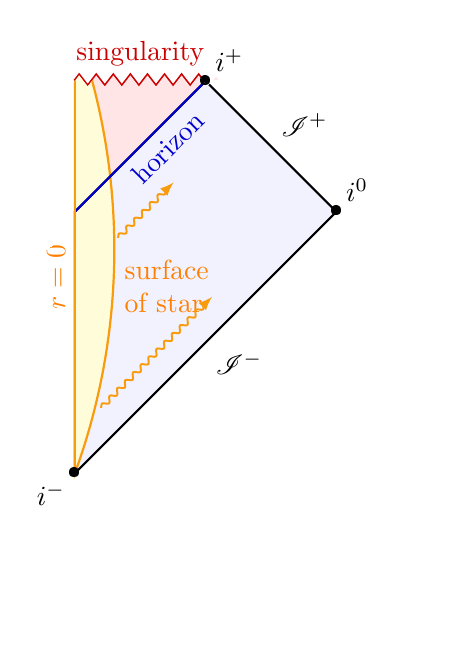
\begin{tikzpicture}

\begin{axis}[axis lines=none, width=1.5*\textwidth,height=1.5*\textwidth, xmin=-5,xmax=5,ymin=-5,ymax=5, disabledatascaling] 

\coordinate[] (O) at (0,0) {};
\coordinate[label = -135:$i^-$] (Ibot) at (0,-2) {};
\coordinate[label = 45:$i^0$] (Iright) at (2, 0) {};
\coordinate[label = 45:$i^+$] (Itop) at (1,1) {};
\coordinate[] (sing) at (0,1) {};


\tikzstyle{singularity}=[red!80!black,line width=1.2,decorate,
                         decoration={zigzag,amplitude=2,segment length=6.17}]


\draw[singularity] (sing) -- node[pos=0.5,above=0] {\strut singularity} (Itop);


\node [black] at (Itop) {\textbullet};

\clip[decorate,decoration={zigzag,amplitude=2,segment length=6.17}]
      (sing) -- (Itop) --++ (1.8,-.2) |-++ (-3,-4) |-++ (0, 4) -- cycle;
\fill[mylightestblue] (Itop) -- (Iright) -- (Ibot) -- (O) -- cycle;
\fill[mylightestred] (sing) |-++ (2,0.1) -- (Itop) -- (O) -- cycle;

\filldraw[fill=mylightyellow, draw=mydarkgold, thick] (Ibot) arc (-20:20:5) node[midway, below right, text width = 1cm, orange] {surface of star} |- (sing) |- (Ibot) |- cycle;

\draw[thick] (Ibot) --
            node[midway, below right]    {$\mathscr{I}^-$}
      (Iright) --
            node[midway, above right]    {$\mathscr{I}^+$}
      (Itop) -- 
      (O) --   
      (Ibot) -- cycle;

\draw[thick, blue!80!black] (Itop) -- 
    node[midway, below, sloped, pos = 0.4] {horizon}
    (O);

\draw[thick, mydarkgold] (Ibot) -- node [midway, above = -.2, sloped, orange] {$r=0$} (sing);

\node [black] at (Itop) {\textbullet};
\node [black] at (Ibot) {\textbullet};
\node [black] at (Iright) {\textbullet};

\coordinate[] (X0) at (0.33, -0.2) {};
\coordinate[] (X1) at (0.2, -1.5) {};

\path 
  (X0) +(45:0.6) coordinate (X0_end);

\path 
  (X1) +(45:1.2)  coordinate (X1_end);

\tikzstyle{photon}=[-{latex},mydarkgold,line width=0.7,decorate,
                    decoration={snake,amplitude=0.9,segment length=4,post length=3.8}]

\draw[->,photon] (X0) -- (X0_end);

\draw[->,photon] (X1) -- (X1_end);

\end{axis}
\end{tikzpicture}
\end{center}


%%%%%%%%%%%%%%%% Tikz Collapsing Star Penrose Diagram %%%%%%%%%%
\vspace{-60pt}
\caption{The Penrose diagram for the Oppenheimer-Snyder model of the collapsing star black hole.}
\label{fig:penrose_collapsing_star}

\end{wrapfigure}

Of course, we still have to make some assumptions to simplify our analysis; in particular, we will assume that the star is perfectly spherically symmetric, and that it collapses with spherical symmetry, too \cite{O_S_blackhole}. We also assume that the star does not rotate, and that it does not dissipate its energy in any way that would allow itself to stabilize during collapse. In other words, the star is presumed to have run out of nuclear energy, meaning it does not produce any more energy from its core, and therefore generates no radiation-based pressure, allowing gravity to compress it rapidly \cite{O_S_blackhole}.

Such a case of pressure-free, spherical collapse is called the \textbf{Oppenheimer-Snyder model} of collapsed-star black hole formation. The Penrose diagram for this case is depicted in Figure 7. Similar to the Schwarzschild case, the collapsing star black hole Penrose diagram also includes a horizon, a ``black hole" region, and a curvature singularity corresponding to $r=0$. It also includes the spacelike, timelike, and lightlike infinites typical of a black hole Penrose diagram on the right side of the diagram.

The similarities end there, however. The first thing we notice is the departure from the ``Penrose diamond" shape for the left hand of the diagram. The past timelike infinity is not spatially aligned with the future timelike infinity, and the past lightlike infinity is represented by a much larger line. Both of these developments can be explained by the third actor in the diagram: the collapsing matter itself.

The orange arc on the diagram represents the \textbf{surface of the collapsing star}, while the yellow region inside represents its \textbf{collapsing matter}. The left end of the diagram represents the center of the star at  $r=0$ \cite{cs_diagram_original}. As the star collapses in on itself (read: bottom to top on the Penrose diagram), it coalesces into a black hole. Unlike the Schwarzschild case where the black hole has always existed, here, some of the time from the past timelike infinity upto a certain point is taken up in the formation of the black hole from the collapsing matter, eventually forming a horizon as is typical of the Schwarzschild case. This is why the bottom end of the diagram \textit{appears} distorted to anyone used to the Schwarzschild case.

We also note that there are two lines corresponding to $r=0$ in this diagram: the center of the star (the leftmost orange line) and the singularity of the formed black hole. Both of these lines have different meanings. The center of the star is \textit{spatially located} at $r=0$ by definition, and hence located at the left end of the diagram. The singularity, on the other hand, represents where all the collapsing matter will \textit{go} after falling into the black hole. In other words, this other ``$r=0$" at the singularity is indicating that once the star has collapsed, all parts of the star not initially at $r=0$ will reach the singularity at $r=0$ \textit{simultaneously} \cite{townsend1997black}, as is indicated by the intersection of the collapsing matter with the singularity at a line at the top end of the diagram.

\begin{wrapfigure}{l}{0.5\textwidth}
\includegraphics[width=0.95\linewidth]{online_CS_bh.png} 
\caption{An alternative Penrose diagram for the Oppenheimer-Snyder model of the collapsing star black hole, where the center of the star ($r=0$) is not aligned vertically (the leftmost purple line). The white line corresponds to the surface of the star, the red line to the horizon, and the cyan line to the singularity \cite{collapse_colorado}.}
\label{fig:penrose_collapsing_star_colorado}

\end{wrapfigure}

The collapsing star Penrose diagram is also useful in that it demonstrates to us what a \textit{real} black hole formation process would look like to an outside observer. Considering two light rays emitted from the collapsing matter, for instance (demonstrated on Figure 7), we notice that the closer we head to the horizon of the formed black hole, the longer it takes for the signal to reach an outside observer in our universe \cite{2022Penrose}. In other words, light from the collapsing star becomes \textit{increasingly redshifted} as it approaches the horizon. The effect is so incredible that we see that light from any matter right at the horizon can only reach the observer after an infinite amount of time, since it will end up at the future timelike infinity. 

Thus, light from matter next to the event horizon will be infinitely redshifted, meaning it will never reach the observer. Overall, this means that to an external observer watching the collapsing star black hole form, they see an infinitely redshifted image of the star corresponding to the moment at which it fell through its event horizon. Over time, the images of the different layers of the star will all coalesce into one at the horizon. \cite{collapse_colorado}. It is important to note, however, that the \textit{black hole has already formed}---its just that this information cannot be conveyed to us in a noninfinite amount of time. From the star's point of view, it has already collapsed to a point and formed a black hole, but we will continue to wait for the light from this event forever.

Overall, then, the collapsing star Penrose diagram is unique in that it demonstrates a process \textit{in action}. In particular, here it displays the process of a star that is collapsing in on itself, meaning that once it passes a certain mass threshold in a certain amount of volume, it forms a black hole, generating an event horizon. 

Recall that the display of an ongoing process on a Penrose diagram is completely permissible---the Penrose diagram, after all, is a representation of both space and \textit{time}. In practice, a Penrose diagram is not a ``snapshot" of spacetime, but rather an evolving system that can be simulated as a process takes place. The Minkowski and Schwarzschild cases we considered earlier did not highlight this point since we assumed in both cases that the spacetimes were eternal. What we see here is an evolving spacetime---one that changes as a black hole forms (hence why the world lines are far too complicated to draw directly on Figure 7).

\section{Conclusion}

Overall, it is clear to see how Penrose diagrams are extremely useful in visualizing spacetimes, and more importantly, performing \textit{causal reasoning} (performing deductions using the properties of lightlike paths). Their utility derives from their role as visual representations of the global causal structure of spacetime---\textit{global} in the sense that they encapsulate all time-like and space-like infinities into a single diagram, and \textit{causal} in the sense that they preserve the property of light traveling at 45 degree angles on the diagram \cite{penrose_colorado}\cite{Dafermos_2005}. 

In achieving these two properties, Penrose diagrams are one of the most powerful tools in the belt of a physicist studying General Relativity. They allow us to understand the complex nature of events near, or within, black holes, where the coordinate and curvature singularities shatter our intuitive understanding of what it means for something to truly be $0$, or \textit{infinite}. By maintaining the properties of the light cone, they also allow us to understand the physicality of geodesics along a spacetime.

The Penrose diagram is therefore a versatile extension to the classic spacetime diagram, yielding impressive results from logical deduction alone. It is truly remarkable that just a few, very simple, coordinate transformations can encapsulate such an insightful geometric representation of spacetimes, all while preserving the underlying, fundamental principles of general relativity.

\printbibliography

\end{document}
